\documentclass[11pt]{article}

\newcommand{\dataset}{{\cal D}}
\newcommand{\fracpartial}[2]{\frac{\partial \#1}{\partial  \#2}}

\usepackage{amsmath,amsthm, amssymb}
\usepackage[all]{xy}
\usepackage{graphicx}
\newtheorem{thm}{Theorem}
\newtheorem{mydef}{Definition}
\usepackage{url}
\usepackage{braket}
\usepackage{listings}
\usepackage{float}
\usepackage{scalefnt}
\usepackage{ifthen}
\usepackage{url}
\usepackage{graphicx}
\usepackage{colortbl}
\usepackage{multirow}
\usepackage{array}

\title{Offer Networks Simulation and Dynamics
	 \\Master's Dissertation Contract}
\author{Zar Goertzel}

\begin{document}
\maketitle

\section{Thesis Statement}
I will run experiments simulating automated transaction suggestions in a moneyless market. The set-up is a network where users upload pairs of tasks they will offer in exchange for requested tasks, which has been called an offer network. I will use either graph or SAT based optimization to find potential transactions, which can be cycles among more than two users. Then I will analyze the network dynamics and performance. If time permits, more features will be experimented with.

\section{Additional Information}
An offer network instance can be represented as a graph where tasks are nodes and directed links represent represent (offer, request) pairs, in which case potential transactions are cycles. Thus finding optimal transaction is a \textbf{maximum vertex cycle problem}. The problem can also be framed in terms of \textbf{weighted boolean optimization}.

\newpage
\section{TODO}

Core goals:
\begin{itemize}
\item Review and summarize related work \\
\item Read up on the state-of-the-art graph / SAT optimizers\\
\item Read up on market performance metrics \\
\item Survey real-world sites to determine realistic initial instances: \newline
	  -- How many users and (offer, request) pairs per user? \newline
	  -- How often will users add new (o, r) pairs?\\
\item Formalize time-complexity of problem \\
\item Formally represent problem instance as graph \\
\item Develop or find and use a problem-instance generator \\
\item Adapt pre-existing optimizer (graph or WBO-based) to problem format \\
\item Finish up simulator via feedback: modify instance by effecting found solution \\
\item Run initial trials and measure: \newline
	-- \% of requests satisfied \newline
	-- average time (iterations?) to being fulfilled \newline
	-- distribution of cycle (match) sizes \newline
	-- ...\\
\item Vary instance parameters (or optimization parameters) and repeat trials \\
\end{itemize}

Extra if time permits:
\begin{itemize}
\item Explore other optimization methods not used above \\
\item Experiment with adding features to the offer network instances, such as gifts (o,) or requests without offers (o,r), or reputation systems \\
\end{itemize}

Questions: 
\begin{itemize}
\item How to view offer network instances and solutions. \\
\item Online vs batch matching -- depends on algorithm \\
\end{itemize}

\section{Timeline}
From 06.02.2017 to about 25.06.2017

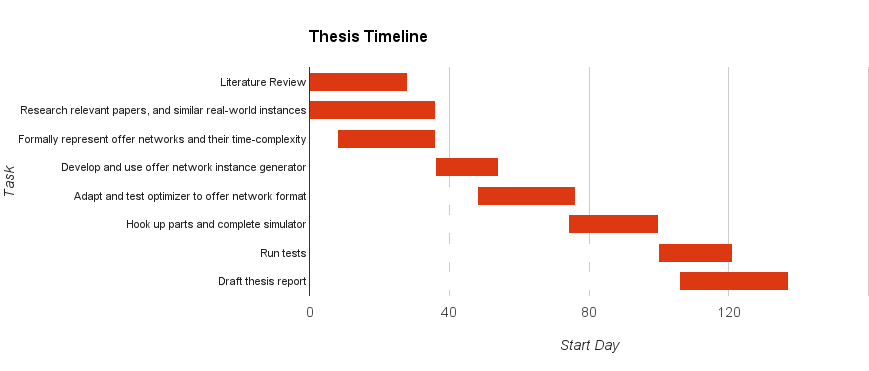
\includegraphics[width=\textwidth]{gantt.png}

\end{document}

